\documentclass{beamer}
\title{Outline}
\usetheme{Hannover}
\setbeamertemplate{footline}[frame number]
\usepackage{amsmath}
\usepackage{amsfonts}
\usepackage{amsthm}
\usepackage{mathtools}
\usepackage[english]{babel}
\usepackage{calc}
\usepackage[absolute,overlay]{textpos}
\usepackage{graphicx}
\usepackage{subfig}
\usepackage{comment}
%\usepackage{tikz}
\usepackage{wasysym}
\usepackage{gensymb}
\usepackage{amssymb}
\usepackage{nccmath}
\usepackage{empheq}
\usepackage{xcolor}
\usepackage{relsize}
\usepackage{multimedia}
\usepackage{media9} 
%\usepackage{natbib}
%\usepackage{apalike}
%\useoutertheme{infolines}


%\setbeamertemplate{sidebar left}{}


% BIB SETTINGS
\usepackage[backend=bibtex,firstinits=true,maxnames=30,maxcitenames=20,url=false,style=authoryear]{biblatex}
%\bibliographystyle{{ieeetr} 
\bibliography{MyBib}
\setlength\bibitemsep{0.3cm} % space between entries in the reference list
\renewcommand{\bibfont}{\normalfont\scriptsize}
\setbeamerfont{footnote}{size=\tiny}
\renewcommand{\cite}[1]{\footnote<.->[frame]{\fullcite{#1}}}

\date{July 05, 2016}

% Insert frame before each subsection (requires 2 latex runs)
\AtBeginSection {
	\begin{frame}<beamer>[noframenumbering] \frametitle{\titleSubsec}
		\tableofcontents[currentsection]  % Generation of the Table of Contents
	\end{frame}
}

% Define the title of each inserted pre-subsection frame
\newcommand*\titleSubsec{Outline}
% Define the title of the "Table of Contents" frame
\newcommand*\titleTOC{Outline}

\setbeamertemplate{navigation symbols}{} % remove navigation symbols

\graphicspath{ {./images/} } 

\begin{document}
%\begin{frame}
%\maketitle
%\end{frame}

\section{Introduction}

\begin{frame}{Introduction}
	\begin{columns}
		\begin{column}{0.6\textwidth}
		Octavio A. Villarreal Maga\~na
		\\
			\begin{itemize}\setlength\itemsep{2.5em}
				\item MSc. Mechanical Engineering, track Control Engineering (TUDelft, The Netherlands)
				\begin{itemize}\setlength\itemsep{1em}
					\item [--] Control Methods for Robotics
					\item [--] Robust Control
				\end{itemize}
				\item BSc. Mechatronic Engineering (UNAM, Mexico)
				\begin{itemize}\setlength\itemsep{1em}
					\item [--] Systems and Control
					\item [--] Robotics
				\end{itemize}
			\end{itemize}
		\end{column}
		\begin{column}{0.4\textwidth}
			\begin{figure}[ht]
				\vspace{-30pt}
				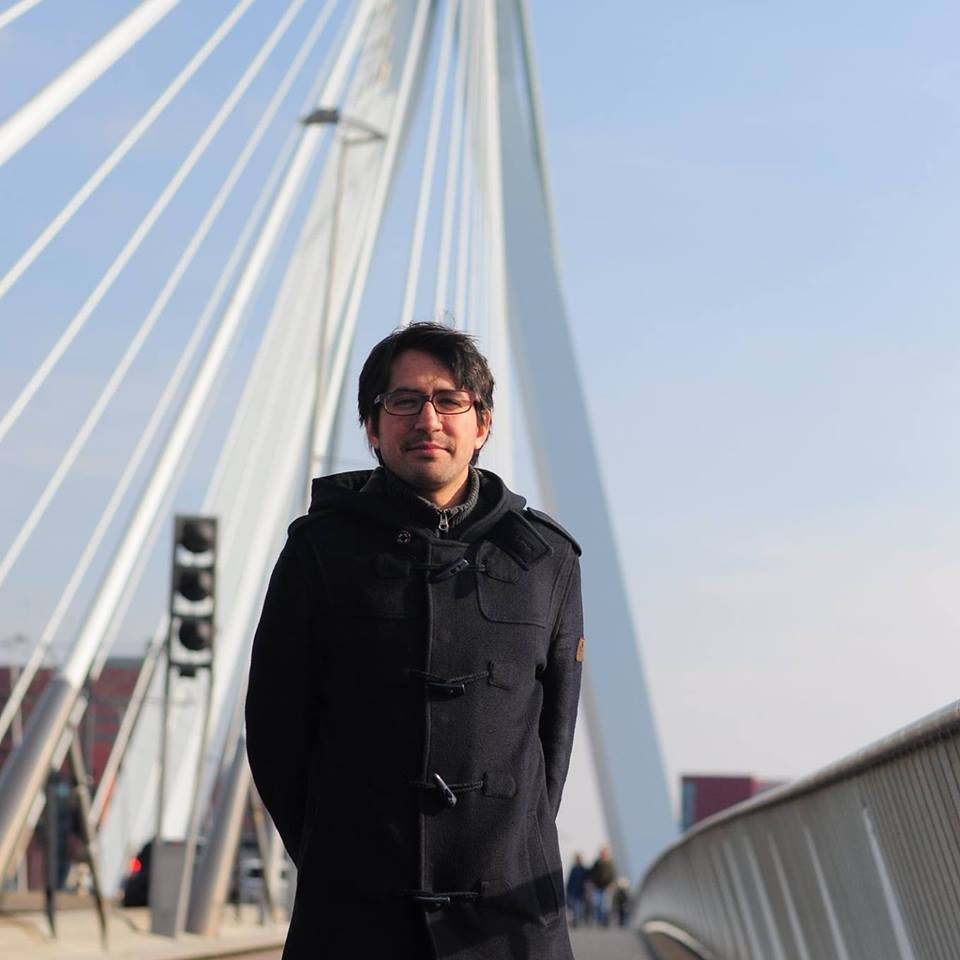
\includegraphics[width=1.5\textwidth]{images/yo.jpg}
			\end{figure}			
		\end{column}
	\end{columns}
\end{frame}

\section{Relevant projects}

%\subsection{Locomotion Control}

\begin{frame}{Locomotion Control of Zebro}
		\begin{columns}
			\begin{column}{0.5\textwidth}
				\begin{itemize}
					\item Course project 
					\item Locomotion control of six-legged robot
					\item Use of max-plus algebra\cite{Lopes2010}
					\item Traversing unstructured terrain
					\item Safe gait switching
				\end{itemize}
			\end{column}
			\begin{column}{0.5\textwidth}
				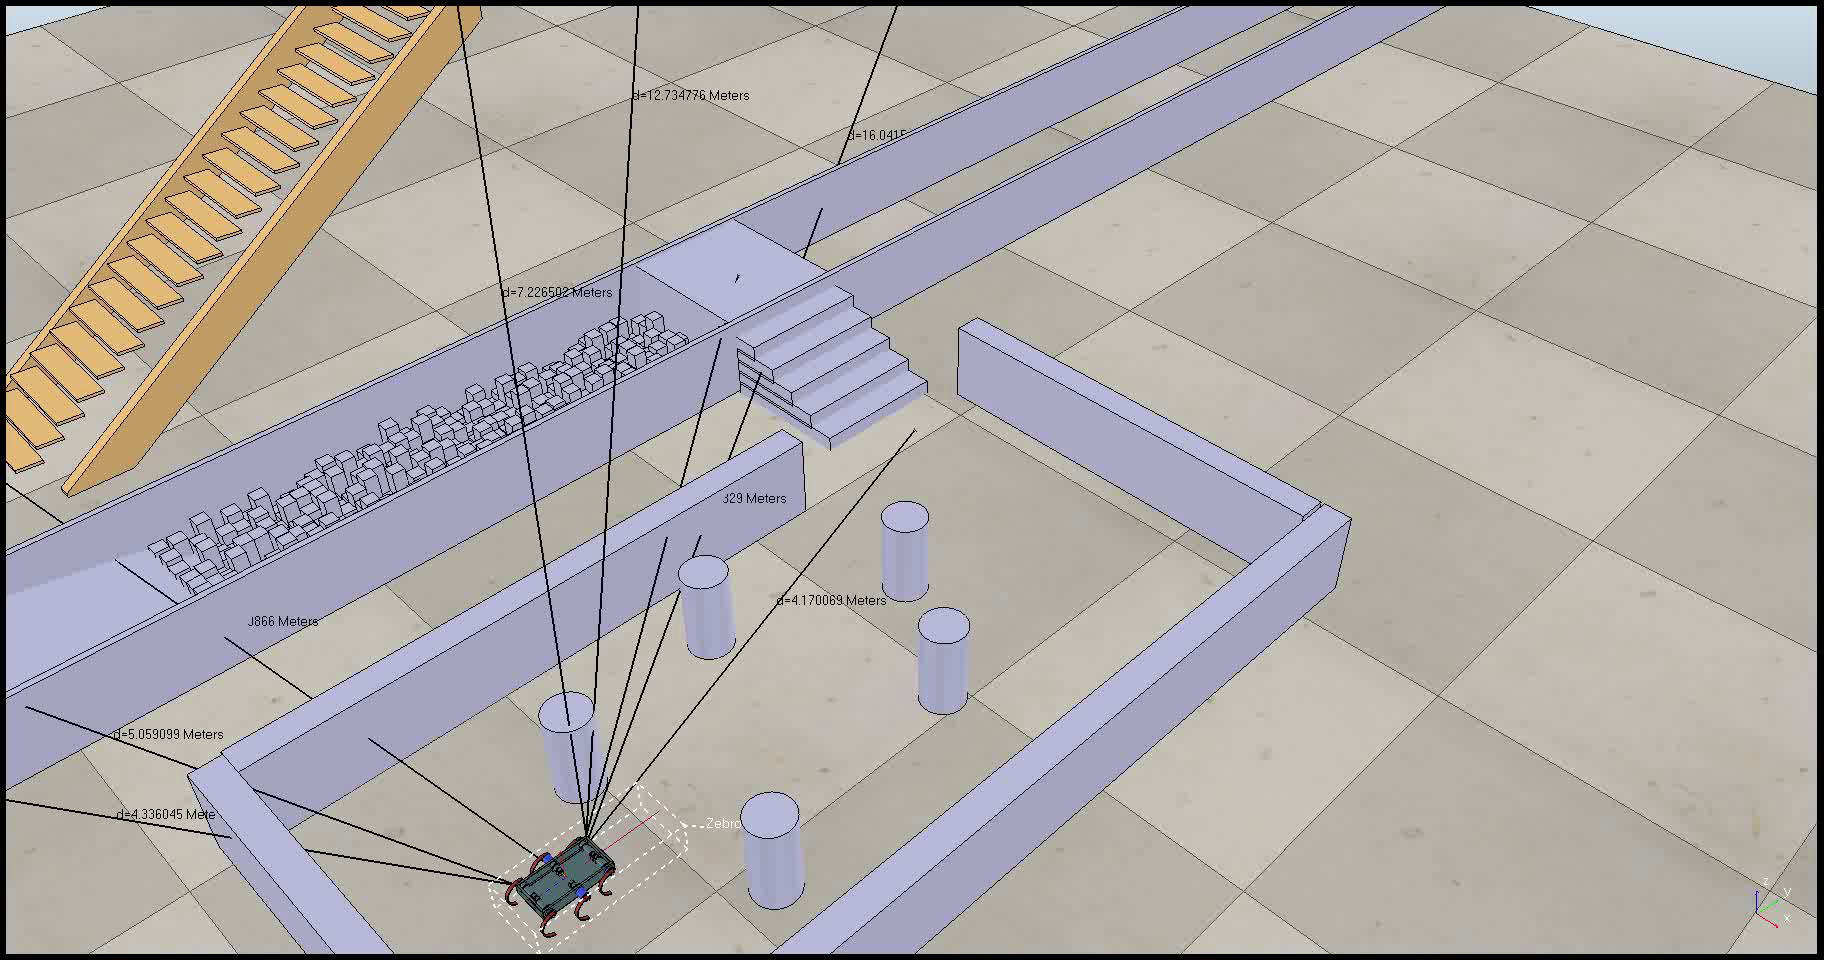
\includegraphics[height=0.55\textwidth]{recording.png}
			\end{column}
		\end{columns}
\end{frame}

\begin{frame}{Implementation in real robot}
	\begin{columns}
				\begin{column}{0.5\textwidth}
					\begin{itemize}
						\item Commissioned by dutch artist
						\item Max-plus algebra for reference generation
						\item Independent controller for each leg
						\item Construction of the robot
						\item Implementation using ROS
						\item Simple obstacle avoidance
					\end{itemize}
				\end{column}
				\begin{column}{0.5\textwidth}
					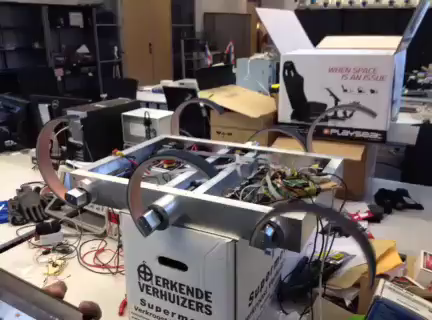
\includegraphics[height=0.7\textwidth]{real.png}
				\end{column}
	\end{columns}
\end{frame}

%\subsection{Master thesis}

\begin{frame}{Robust output-feedback control of 3D directional drilling systems}
	\begin{columns}
		\begin{column}{0.5\textwidth}
			\begin{itemize}
			\item MSc Thesis 
			\item In collaboration with the University of Minnesota
			\item Complex dynamics (Delay Differential Equations)
			\item Observer design to only use local measurements
			\item Robust against parameter uncertainty
			\end{itemize}
		\end{column}
		\begin{column}{0.5\textwidth}
			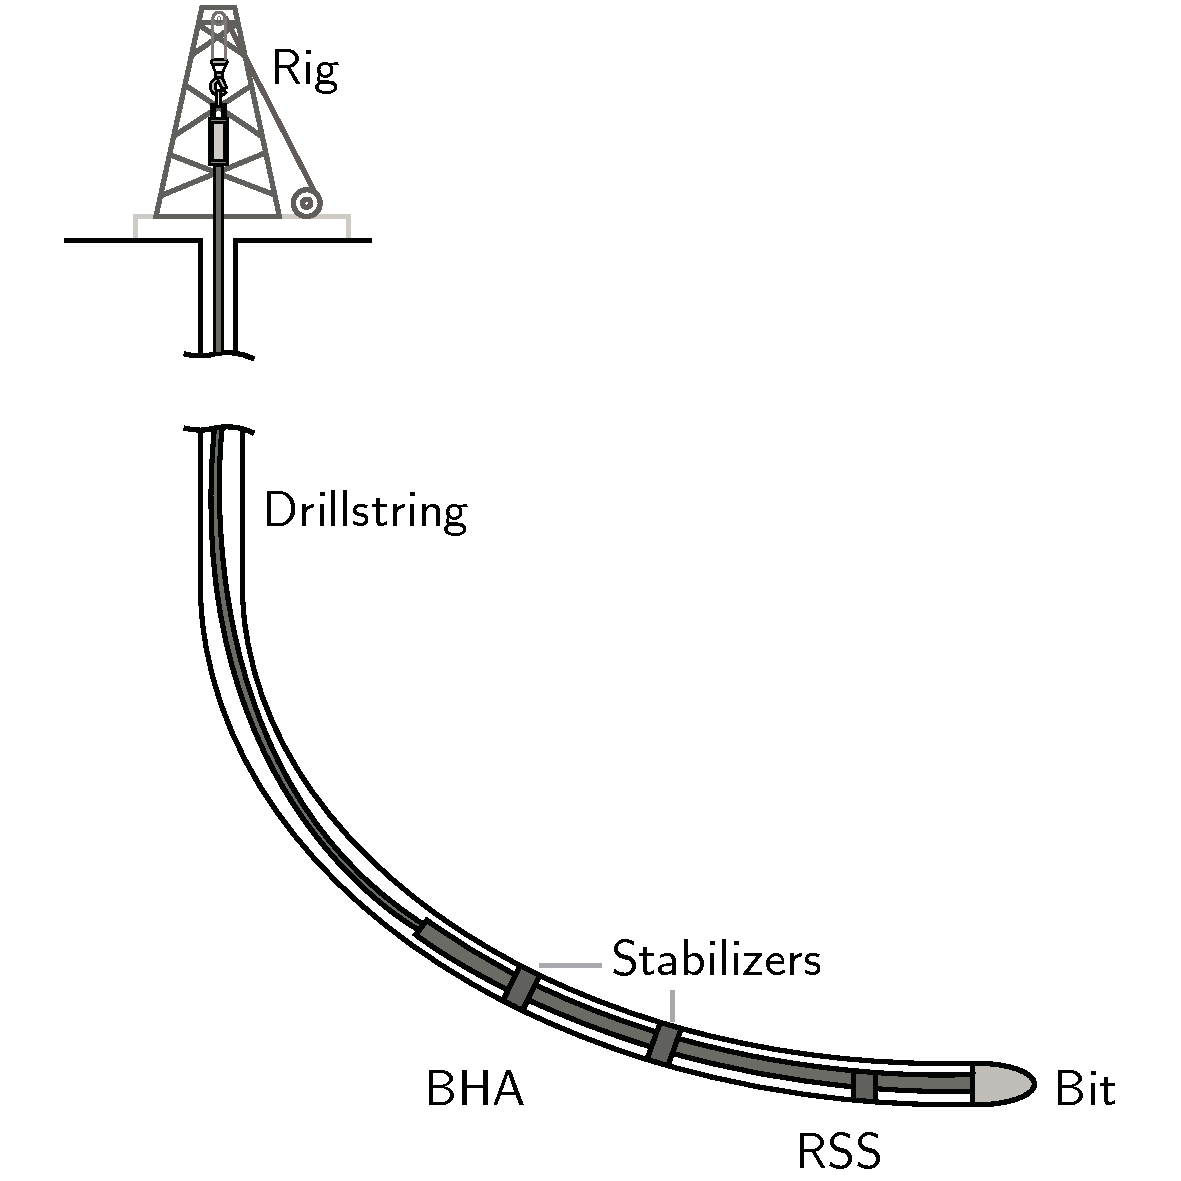
\includegraphics[width = 1\textwidth]{drillingsystem.pdf}
		\end{column}
	\end{columns}
\end{frame}

%\subsection{Control of robotic arm}

\begin{frame}{Control of robotic arm}
	\begin{columns}
		\begin{column}{0.5\textwidth}
			\begin{itemize}\setlength\itemsep{2.5em}
			\item Control Methods for Robotics course assignment
			\item Four rotational joints
			\item Different control algorithms (Workspace and configuration space control)
			\end{itemize}
		\end{column}
		\begin{column}{0.5\textwidth}\centering
			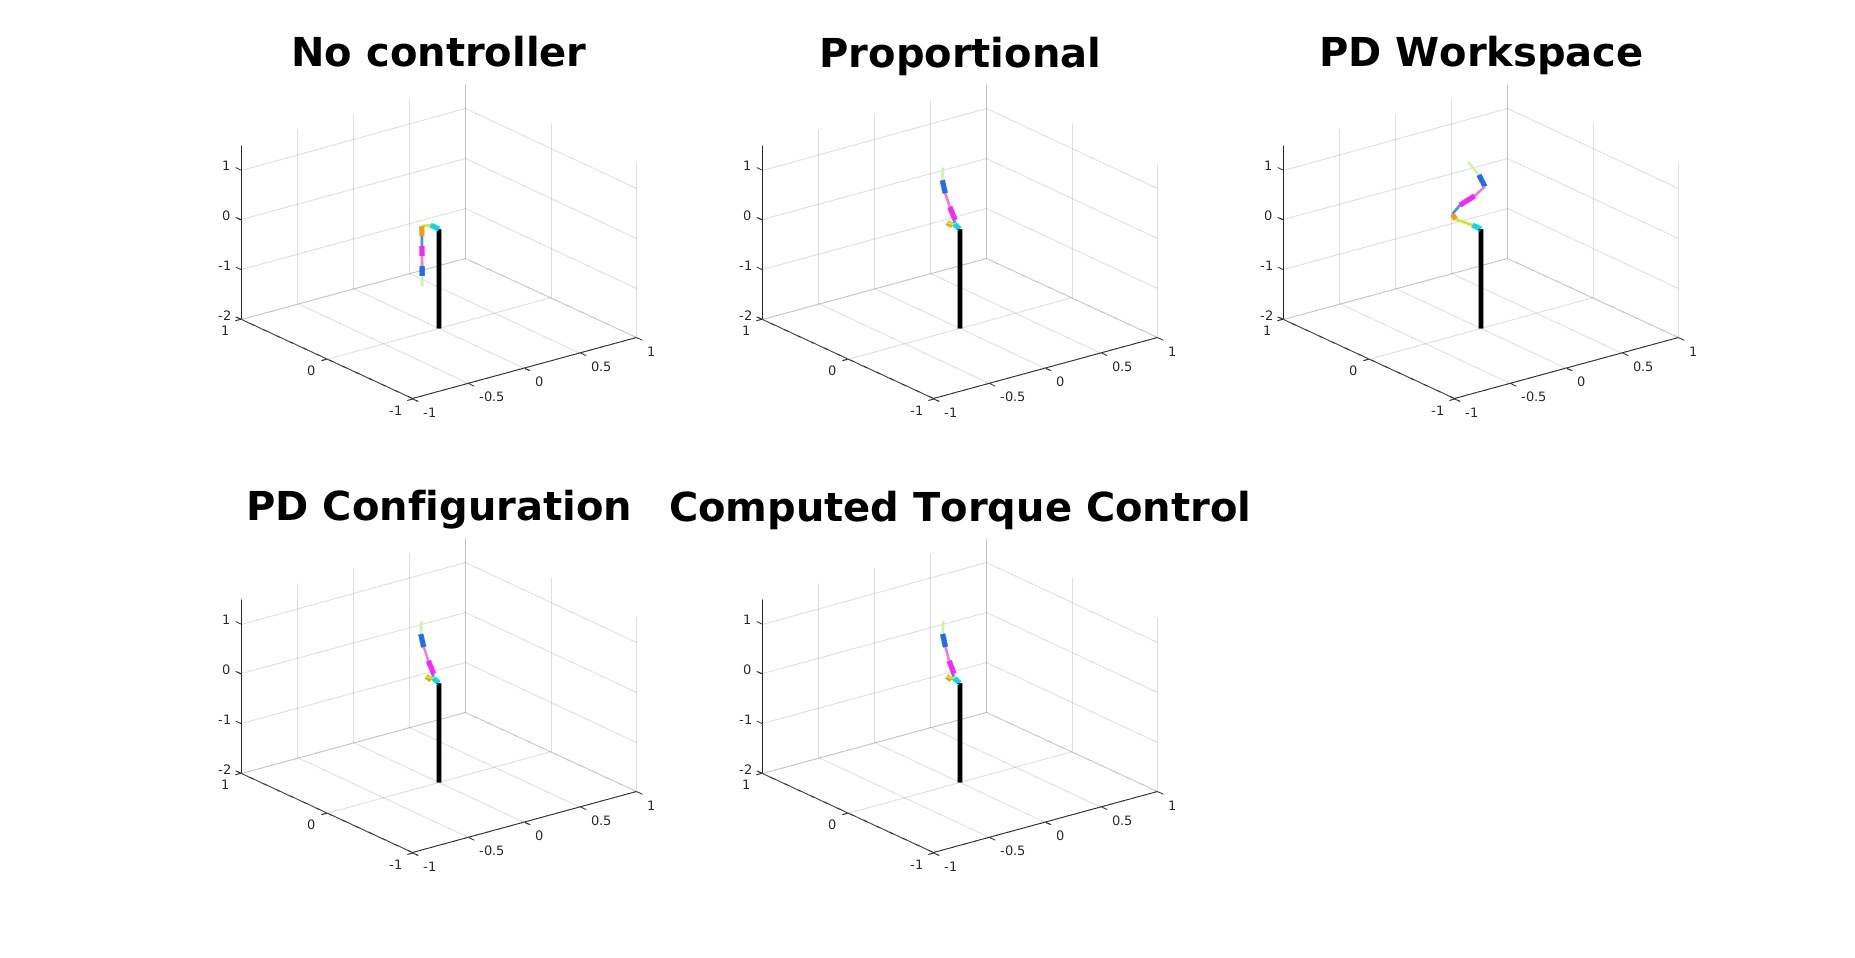
\includegraphics[height = 0.55\textwidth]{Robot.png} \\
			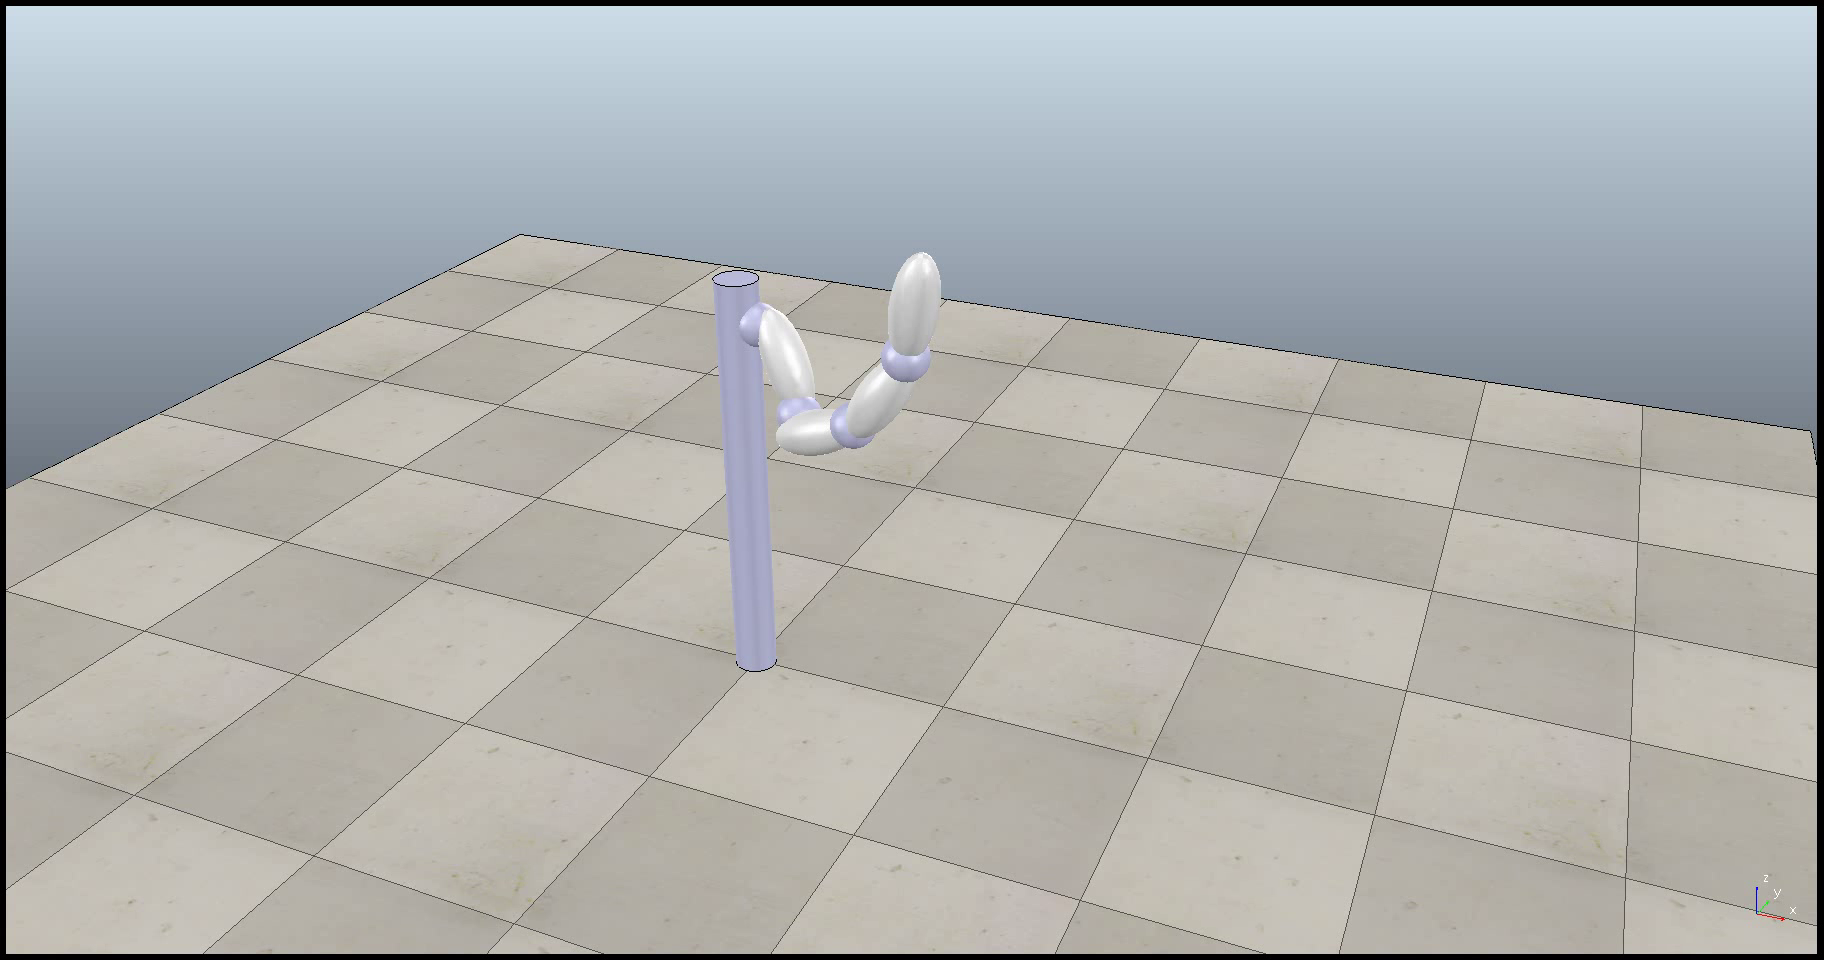
\includegraphics[height=0.5\textwidth]{recording2.png}
		\end{column}
	\end{columns}
\end{frame}

%\subsection{Control of quadcopter}
			
\begin{frame}{Nonlinear geometric control of quadcopter}
\begin{columns}
	\begin{column}{0.5\textwidth}
		\begin{itemize}\setlength\itemsep{2.5em}
			\item Control Methods for Robotics course assignment
			\item Workspace and orientation nonlinear control
			\item Capable of performing aggresive maneuvers\cite{Quad}
		\end{itemize}
	\end{column}
	\begin{column}{0.5\textwidth}
			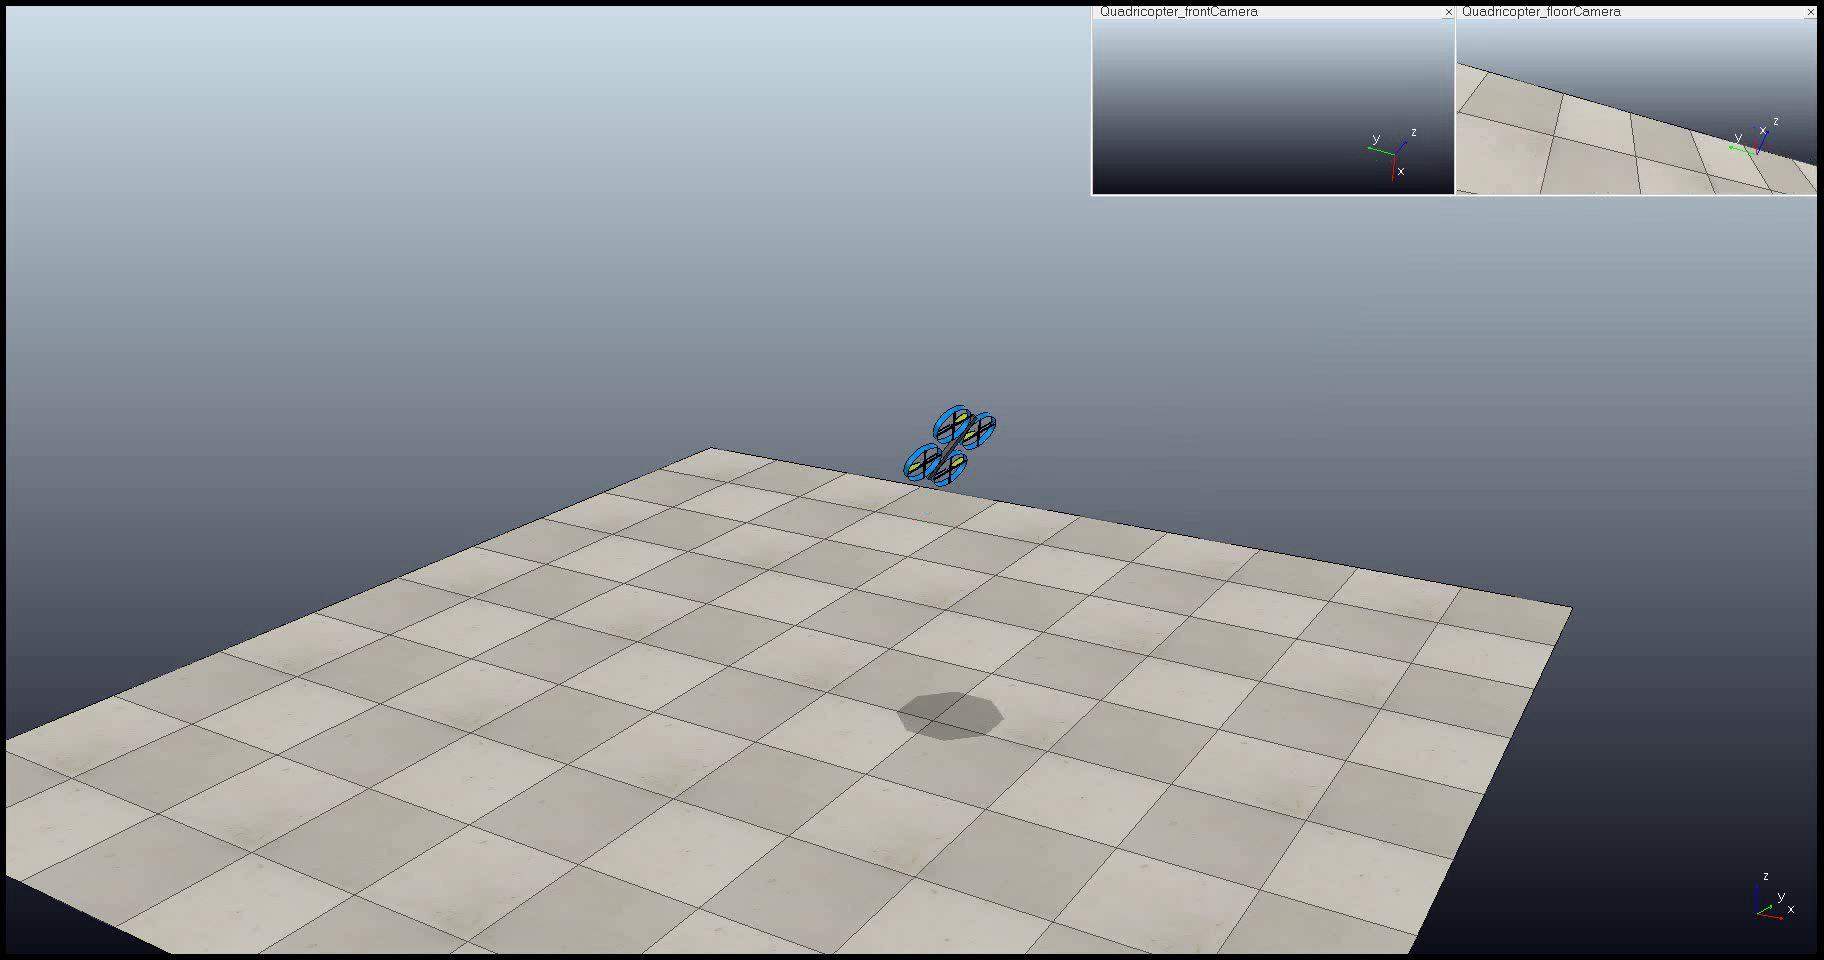
\includegraphics[height=0.55\textwidth]{recording3.png}
	\end{column}
\end{columns}
\end{frame}	

\section{Research proposal}

%\subsection{Preliminaries}

\begin{frame}{Objective of max-plus algebra in locomotion}\textbf{"Obtain synchronized time references for each of the leg's lift-off times (moment when a leg leaves the ground) and touch-down times (moment when a leg touches the ground)  in a systematic way".}
\end{frame}

\begin{frame}{Definition of max-plus algebra}

"Tropical" algebra defined by:
	
	\begin{equation*}
		(\Re_{max}, \oplus, \otimes, \varepsilon, e)
	\end{equation*}
	
	where:
	
	\begin{align*}
		\Re_{max} &:= \Re \cup \{-\infty\}, \nonumber\\
		x \oplus y &:= max(x,y), \nonumber\\
		x \otimes y &:= x + y, \nonumber\\
		\varepsilon &:= -\infty, \nonumber\\
		e &:= 0. \nonumber
	\end{align*}
\end{frame}

\begin{frame}{Definition of max-plus algebra}
\vspace{20pt}
Extension to matrices:
\begin{equation*}
		(\Re_{max}^{n\times m}, \oplus, \otimes,\mathcal{E}, E)
	\end{equation*}
	
	with:
	
	\begin{align*}
		[A \oplus B]_{ij} &= a_{ij} \oplus b_{ij} := \max(a_{ij},b_{ij}), \nonumber \\
		[A \otimes C]_{ij} &= \underset{k=1}{\overset{m}{\mathlarger{\mathlarger\oplus}}}a_{ik} \otimes c_{kj} := \max\limits_{k=1,...,m}(a_{ik} + c_{kj}), \nonumber 
	\end{align*}
	Absorbing and identity element:
	\begin{align}
			[\mathcal{E}]_{ij} &= \varepsilon, \nonumber \\
			[E]_{ij} &= \begin{cases}
				e, & \text{if } i =j \\
				\varepsilon,& \text{otherwise.}
			\end{cases} \nonumber
		\end{align}
	Powers:
	\begin{equation*}
			D^{\otimes k} := D \otimes D \otimes... \otimes D.
	\end{equation*}
\end{frame}

%\subsection{Gait generation}
\begin{frame}{Gait generation using max-plus algebra}
Gait Parameters\cite{Lopes2010}:
\begin{table}[ht]
		\label{table:Parameters}
		\begin{tabular}{ll}
			\color{blue}$i$           & Leg index.                                                            \\
			\color{blue}$t_i (k)$     & Touchdown time of leg.                                                                     \\
			\color{blue}$l_i (k)$     & Lift-off time.                                                                      \\
			\color{blue}$\tau$        & Current time instant.                                                                          \\
			\color{blue}$\tau_f$      & Flight time.                                                             \\
			\color{blue}$\tau_g$      & Ground time.                                                        \\
			\color{blue}$\tau_\Delta$ & Double stance time (adjustable).
		\end{tabular}
	\end{table}
\end{frame}

\begin{frame}{Gait generation using max-plus algebra}
	Gait cycle description for a biped:
	\begin{align*}
			t_1 (k+1) &= l_1 (k+1) + \tau_f \\
			l_1 (k+1) &= t_1 (k) + \tau_g \\
			t_2 (k+1) &= l_2 (k+1) + \tau_f \\
			l_2 (k+1) &= t_2 (k) + \tau_g
	\end{align*}
	Synchronization:
	\begin{align*}
			t_1 (k+1) &= l_1 (k+1) + \tau_f \\
			l_1 (k+1) &= \color{blue}\max (\color{black}t_1 (k) + \tau_g\color{blue},t_2(k) + \tau_\Delta)\\
			t_2 (k+1) &= l_2 (k+1) + \tau_f \\
			l_2 (k+1) &= \color{blue}\max (\color{black}t_2 (k) + \tau_g\color{blue},t_1(k+1) + \tau_\Delta)
		\end{align*}
\end{frame}

\begin{frame}{Gait generation using max-plus algebra}
	Described as a max-plus linear system:
	\begin{equation*}
		\underbrace{	\begin{bmatrix}
		t_1 (k+1) \\
		t_2 (k+1) \\
		l_1 (k+1) \\
		l_2 (k+1)
		\end{bmatrix}}_{x(k+1)} = 
		\underbrace{\begin{bmatrix}
		\tau_f \otimes \tau_g & \tau_f \otimes \tau_\Delta 	& \varepsilon & \varepsilon \\
		\tau_f^{\otimes 2} \otimes \tau_g \otimes \tau_\Delta & (\tau_f \otimes \tau_\Delta)^{\otimes 2} & \varepsilon & \varepsilon \\
		\tau_g & \tau_\Delta & \varepsilon & \varepsilon \\
		\tau_f \otimes \tau_g \otimes \tau_\Delta & \tau_f \otimes \tau_\Delta^{\otimes 2} & \varepsilon & \varepsilon
		\end{bmatrix}}_{A}
		\underbrace{\begin{bmatrix}
			t_1 (k) \\
			t_2 (k) \\
			l_1 (k) \\
			l_2 (k)
		\end{bmatrix}}_{x(k)}
	\end{equation*}
	Gait definition:
	\begin{align*}
		\mathcal{G}_{walk} &= \{1\} \prec \{2\} \\
		\mathcal{G}_{hop} &= \{1,2\}
	\end{align*}
\end{frame}

\begin{frame}{Advantages}
	\begin{itemize}
		\item Systematic gait generation
		\item Number of legs does not increase complexity greatly
		\item Safe gait switching \cite{Lopes2009}
		\item Total cycle-time, steady-state and transient behavior analysis by studying properties of $A$ matrix
	\end{itemize}
\end{frame}

%\subsection{Locomotion control}

\begin{frame}{Locomotion control of walking robots}
	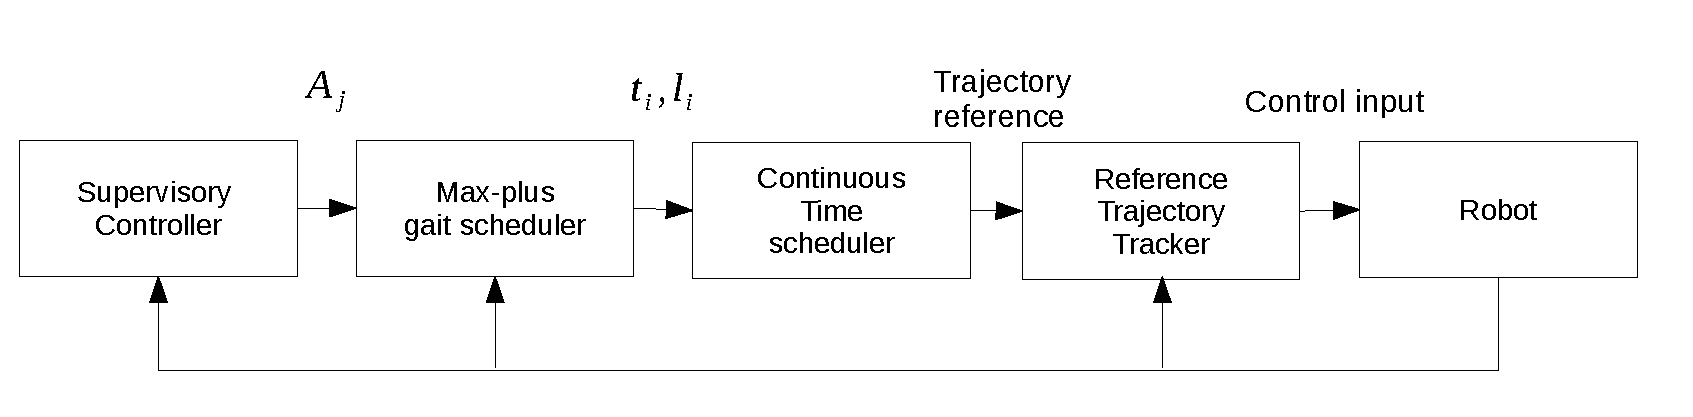
\includegraphics[width=1\textwidth]{images/Control.pdf}
\end{frame}

\begin{frame}{Locomotion control of walking robots}
	\begin{itemize}\setlength\itemsep{1.5em}
			\item Supervisory control : Defines $A_j$ matrix ($\tau_g$, $\tau_f$, $\tau_\Delta$,etc.)
				\begin{itemize}
				\item [--] Uses sensor information
				\end{itemize}
			\item Gait scheduler: Defines lift-off and touch-down times for each leg (final and initial times for trajectory)
			\item Continuous time scheduler: Defines trajectory for each of the legs based on scheduled times
				\begin{itemize}
				\item [--] For example, an ellipsoidal trajectory
				\end{itemize}
			\item Reference trajectory tracker: Follows the trajectory defined
				\begin{itemize}
				\item [--] e.g. workspace computed torque control
				\end{itemize}
		\end{itemize}
\end{frame}

\section{Expected results}

\begin{frame}{Expected results}
	\begin{itemize}\setlength\itemsep{1.5em}
		\item Systematic method to generate gaits
		\item Methodology could provide safe gait switching
		\item Could be applied to several topologies of multi-legged robots
		\item Could provide robustness against unstructured scenarios
	\end{itemize}
\end{frame}

\end{document}